\subsection{Coverage, local amortization, and complete solves}

The retained coverage battery uses camera, Barbara, a histogram-preserving camera permutation, a straight carrier, and crossing carriers with an edge, all at $64\times64$. Ordinary anchors are taken after $4,32,128,512$ passes, with depths $2,4,8$ and horizons $8,16,32,64$. All 240 measured quotient errors satisfy \eqref{eq:curvedpath} within numerical tolerance. The texture errors after settling are independently checked as well. The certificate is an analytic bound; these finite tests verify its implementation rather than establish the theorem.

For example, at camera prefix $512$, depth two and horizon sixteen, the bound is $0.0954$ times predicted displacement and the actual error is $0.019$ times actual displacement. At camera prefix four the same horizon has a much larger curvature budget. Increasing depth can reduce compression without removing that changing geometry.

The live discovery policy acquires depths $2,4,8$ incrementally and checks the reduced path in chunks of eight up to horizon $64$. It stops a depth after the first chunk whose accumulated bound exceeds $0.1$ times predicted displacement, then selects a checked horizon whose nominal operator savings exceed $1.5\times$ acquisition and settling work. This early stopping rule need not find the longest admissible horizon. It does not consult a future trajectory or gap oracle.

The policy accepts seven of the twenty anchors. With five timing repeats, the late camera block discovers depth two/horizon sixteen and is $1.39\times$ faster than ordinary replay. The straight carrier at prefixes $128$ and $512$ discovers depth two/horizon sixty-four and gives $3.47\times$ and $3.48\times$ speedups. Three of the seven accepted blocks are slower despite passing the nominal work screen. Timings include chart acquisition, radial checks, reconstruction, and one settling pass for both methods.

\begin{figure}[htbp]\centering

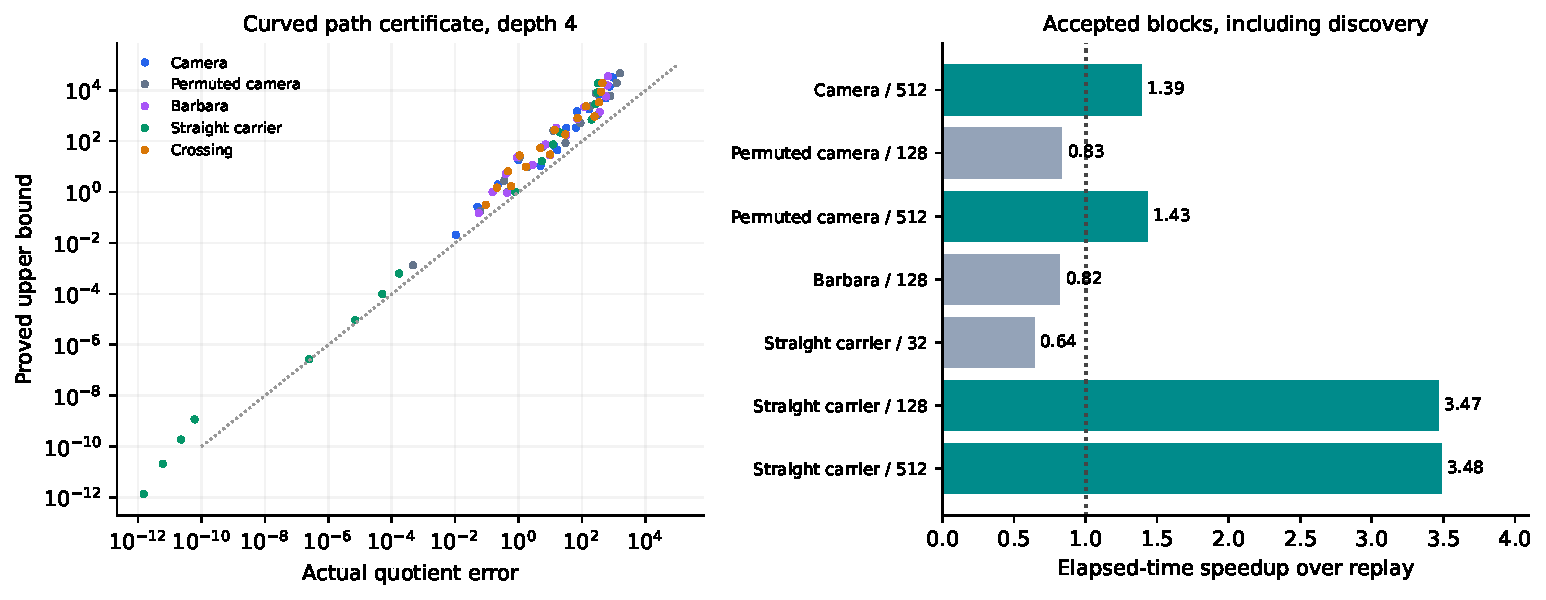
\includegraphics[width=\textwidth]{figures/curved_validity.pdf}

\caption{Left: independently replayed errors and the curved certificate for depth four, across all anchors and horizons. The dotted diagonal is equality; plotting floors are $10^{-12}$. Right: all seven accepted live-discovery blocks, labeled by source and ordinary anchor prefix. Thirteen rejected anchors remain in the raw records.}

\end{figure}

For complete solves, all methods use the same original recurrence and the same recovered primal--dual gap. The target is $10^{-4}$ times the initial gap, checked every thirty-two work units. The fixed methods use depth four, horizon sixteen, and one settling pass; they differ only in six-field Euclidean versus whitened quotient coordinates. The discovered method takes thirty-two ordinary steps after an unprofitable acquisition. Its fallback also charges an additional pass to recover the full primal output. The work ceiling is 4096; all methods reach the target on every source.

\begin{table}[htbp]\centering\small

\begin{tabular}{l rrrr}\toprule

Source & Ordinary & Fixed, six fields & Fixed, quotient & Discovered\\\midrule

Camera & 229.9 & 407.7 & 419.9 & 386.3\\

Permuted camera & 32.8 & 78.9 & 76.0 & 63.4\\

Barbara & 98.2 & 154.1 & 174.3 & 187.2\\

Straight carrier & 24.6 & 36.7 & 46.4 & 53.6\\

Crossing & 174.8 & 172.2 & 263.2 & 279.7\\

\bottomrule\end{tabular}

\caption{Complete Python solve milliseconds on the M4 Mini, one BLAS thread, median of three shuffled timed runs after warm-up. Setup is excluded; gap checks, discovery, rejected candidates, and all update work are included. These are not native-kernel timings.}

\label{tab:curvedsolve}\end{table}

The conservative discovered policy loses to ordinary iteration on all five complete solves, despite profitable certified blocks in some later regimes. This is a retained negative result. A valid curved description is now available for the original map; the current acquisition policy and sufficient path-error bound are not yet an economical general accelerator. As in the earlier Meyer probe, successful acceleration need not closely reproduce the entire ordinary trajectory. The strict certificate is a controlled research instrument, not a replacement imposed on the established native operator.

The continuation suite passes 41 tests, including the exact future-driving quotient, the stronger averaged-map inequality, curvature formulas across boundary events, sharp attainment of the Fourier response gain, and independently replayed path bounds.
